\section*{Introduction}
Dans ce chapitre, nous présenterons quelques travaux antérieurs dans le domaine
de la transcription automatique de la musique et de la batterie afin de situer
notre démarche.

Nous aborderons le passage crucial du monophonique au polyphonique dans la
transcription. Nous ferons un point sur les deux grandes parties de la TAM de
bout en bout : de l’audio vers le MIDI puis des données MIDI vers l’écriture
d’une partition. Ensuite, nous discuterons des approches linéaires et des
approches hiérarchiques.

\section{Monophonique et polyphonique}
Les premiers travaux en transcription ont été faits sur l’identification des
instruments monophoniques\footnote{Instruments produisant une note à la fois,
ou plusieurs notes de même durée en cas de monophonie par accord (flûte,
clarinette, sax, hautbois, basson, trombone, trompette, cor, etc…)}
\cite{future_directions}. Actuellement, le problème de l'estimation automatique
de la hauteur des signaux monophoniques peut être considéré comme résolu, mais
dans la plupart des contextes musicaux, les instruments sont polyphoniques
\footnote{guitare, piano, basse, violon, alto, violoncelle, contrebasse,
glockenspiel, marimba, etc…}. L'estimation des hauteurs multiples est le
problème central de la création d'un système de transcription de musique
polyphonique. Tout signal audio musical peut être composé de plusieurs signaux,
ceux-ci pouvant provenir de plusieurs instruments, ou d'un instrument dit
polyphonique. Une tâche difficile consiste à séparer, à partir du signal, les
différentes sources (ou voix) afin de les représenter individuellement. La
batterie, composée de plusieurs instruments (caisse claire, grosse caisse,
cymbales, toms, etc…), est un cas typique d'intrument polyphonique pour lequel
ce défi est majeur .

Les performances des systèmes actuels ne sont pas encore suffisantes pour
permettre la création d'un système automatisé capable de transcrire de la
musique polyphonique sans restrictions sur le degré de polyphonie ou le type
d'instrument. Cette question reste donc encore ouverte.

\section{De l’enregistrement audio vers le MIDI}
\label{audio_to_midi}
Jusqu’à aujourd’hui, les recherches se sont majoritairement concentrées sur le
traitement de signaux audio vers la génération de contenu MIDI non-quantifié
(une performance — à expliquer) \cite{AMT_for_2_Instru}. Cette tâche englobe
plusieurs sous-tâches dont séparation des sources audio, la détection
multi-\textit{pitchs} \footnote{La détection multi-\textit{pitchs} est la
détection des hauteurs simultanées pour les instruments polyphoniques. Il peut
s’agir de notes d’un même instrument ou de plusieurs instruments différents.}
et la détection des \textit{onsets} et des \textit{offsets}.

\florent{avant la TAB, il faudrait dire 2 mots sur les techniques utilisées
(cf. survey AMT Benetos et al.)}

En transcription automatique de la batterie \cite{Review_ADT}, plusieurs
stratégies de répartition pré/post-\textit{processing} sont possibles pour la
détection multi-\textit{pitchs}. La détection peut être entamée dès le
pré-\textit{processing}, en supprimant les \textit{features}\footnote{
Features : caractéristiques individuelles mesurables d'un phénomène dans le
domaine de l'apprentissage automatique et de la reconnaissance des formes}
non-pertinentes pendant la séparation des sources afin d’obtenir une meilleure
détection des instruments de la batterie, par exemple en supprimant la
structure harmonique pour atténuer l’influence des instruments à hauteurs sur
la détection grosse caisse et caisse claire. Mais certaines études montrent que
la suppression des instruments à hauteurs peut avoir des effets néfastes sur
les performances de la transcription de batterie. En outre, les systèmes de TAB
basés sur des réseaux de neurones récurrents ou sur des factorisations
matricielles font la séparation des sources pendant l’optimisation, ce qui
réduit la nécessité de la faire pendant le pré-processing. Pour la
reconnaissance des instruments de la batterie, une autre approche possible est
d’utiliser un modèle probabiliste (MMC) pour classifier les différents sons de
la batterie \cite{Eronen}. L’approche AdaMa \cite{adama_1}, qui commence par
une estimation initiale des sons de la batterie en les raffinant itérativement,
est une autre approche de la même catégorie.

Toutes ces méthodes elles visent toutes la génération d’un contenu MIDI
non-quantifié qui est la représentation symbolique d’une performance musicale.

\section{Du format MIDI vers une partition}
Les approches mentionnées en section \ref{audio_to_midi} produisent en sortie
un fichier MIDI non-quantifié, qui est un format encore très éloigné d'une
partition musicale. Un premier problème concerne les timings (dates et durées
d'événements) qui doivent être alignées à des positions temporelles
correspondant à des valeurs exprimables avec la notation musicale (voir la
différence entre contenu MIDI et musique écrite en section 1.4). On parle de
quantification rhythmique.

Nakamura et al. 2016 présentent une approche de quantification rhythmique avec
modèles de probabilités (MMC) qui prend en entrée un fichier MIDI non quantifié
et fourni en sortie un fichier MIDI quantifié. \cite{SHIBATA2021262} étendent
ensuite l'approche à une transcription d'enregistrement audio vers un fichier
MIDI quantifié. Ce dernier format, linéaire, ne correspond toutefois pas encore
à une partition structurée,  avec groupement rythmiques hérarchiques (voir la
section 1.4). Dans ces travaux, la structuration des données en partition est
déléguée à un éditeur de partitions (MuseScore), avec des résultats assez
inégaux.

Seuls quelques travaux récents s’intéressent de près à la création d’outils
permettant la génération de partition. Le problème de la conversion d'une
séquence d'évènements musicaux symboliques en une partition musicale structurée
est traité notamment dans \cite{foscarin:hal-01988990}. Ce travail, qui vise à
résoudre de manière conjointe la quantification rythmique et la production de
partitions structurées, s’appuie tout au long du processus sur des grammaires
génératives qui fournissent un modèle hiérarchique — langage a priori des
partitions. Les expériences ont des résultats prometteurs, mais il faut relever
qu’elle ont été menées avec un ensemble de données composé d'extraits
monophoniques ; Il reste donc à traiter le passage au polyphonique, qui
nécessite de traiter le problème supplémentaire de la séparation de voix,
\florent{i.e. pour la batterie on nveut quantification + structuration +
    séparation mais seules les 2 premières sont couplées dans l'approche de
    ton stage.}
en le couplant avec la quantification du rythme.

L'approche de \cite{foscarin:hal-01988990} est fondée sur la conviction 
que la complexité de la structure musicale dépasse les modèles linéaires.

\section{Approche linéaire et approche hiérarchique}

\begin{figure}[h]
	\centering
	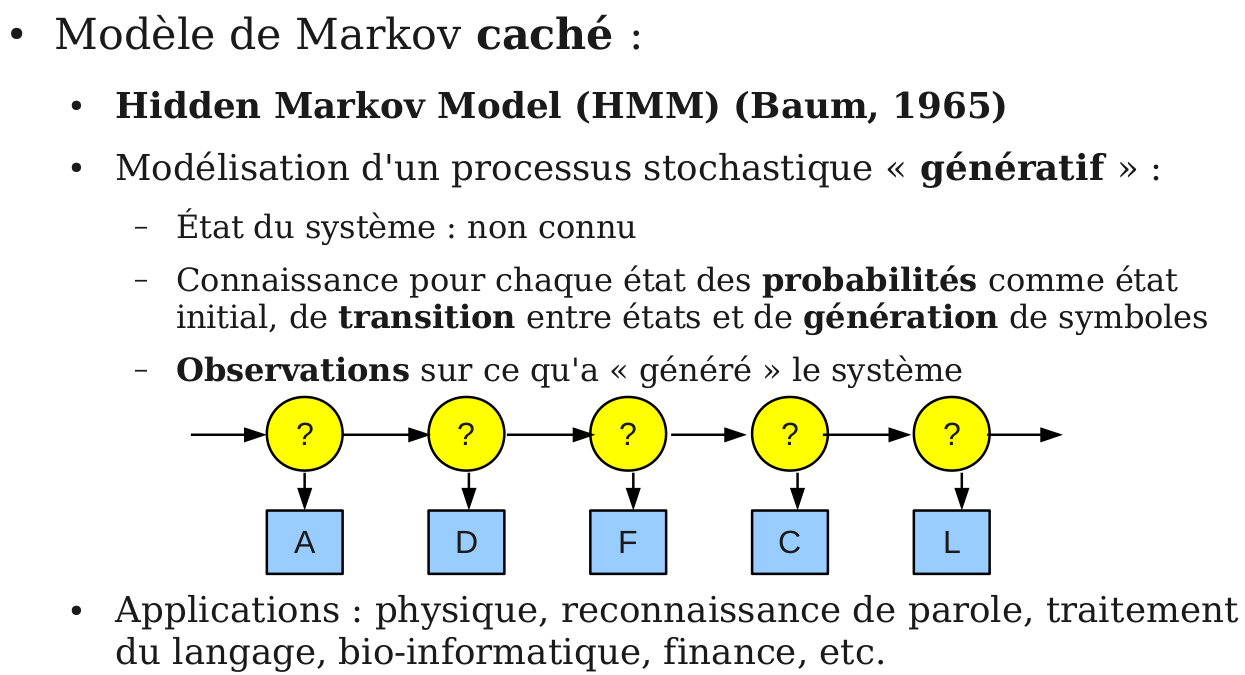
\includegraphics[height=50mm, width=90mm]{
    z_images/2_etat_de_l_art/0_hmm.png}
	\caption[Le modèle de Markov caché]{Le modèle de Markov caché\footnotemark}
    \label{mmc}
\end{figure}

<dam>qu'est-ce q'un modèle linéaire</dam>\\
La figure \ref{mmc} montre un exemple de modèle linéaire et mentionne notamment
ce type de modèle sont utilisé en reconnaissance de la parole. Une différence
notable entre la reconnaissance de la parole et le traitement de la musique est
que la parole est un type de données linéaires : les informations sonores
arrivent les unes après les autres. Mais l’expression musicale provient en
grande partie du mélange des sons. Certaines information musicales sont
nécessairement issues de plusieurs sons produit simultanément.

Plusieurs travaux ont d’abord privilégié l’approche stochastique. Par exemple,
Shibata \textit{et al.} \cite{SHIBATA2021262} ont utilisé des MMC pour la
reconnaissance des signatures rythmiques. Les auteurs utilisent d’abord deux
réseaux de neurones profonds, l’un pour la reconnaissance des \textit{pitchs}
et l’autre pour la reconnaissance de la vélocité. Ils construisent ensuite
plusieurs MMC étendus pour la musique polyphonique correspondant à des
signatures rythmiques possibles, puis ils calculent la probalitité maximale
pour chaque modèle afin d’obtenir la signature rythmique la plus probable.\\

L’évaluation finale des résultats de \cite{SHIBATA2021262} montre qu’il faut
\footnotetext{Source : cours de Damien Nouvel
\url{https://damien.nouvels.net/fr/enseignement}}
rediriger l’attention vers les valeurs des notes, la séparation des voix et
d'autres éléments délicats de la partition musicale qui sont significatifs pour
son interprétation.

Même si la quantification du rythme se fait le plus souvent par la
manipulation de données linéaires, de nombreux travaux suggèrent d’utiliser
une approche hiérarchique puisque le langage musical est lui-même structuré.

\florent{je ne comprend pas bien l'explication. le pb est plutot vue locale 
(déduction de la proba d'une durée à partir de la durée précédente, par ex.
dans un MMC) 
vs vue globale, dans une hiérarchie}

En effet, l’usage d’arbres syntaxiques semble approprié pour représenter le
langage musical. Une méthodologie simple pour la description et l'affichage des
structures musicales est présentée dans \cite{rythm_tree}. 
Les arbres de rythmes y sont évoqués comme permettant une cohésion complète de
la notation musicale traditionnelle avec des notations plus complexes.
Jacquemard \textit{et al.} \cite{jacquemard:hal-01134096} propose aussi une
représentation formelle du rythme, inspirée de modèles théoriques antérieurs
issus du domaine de la réécriture de termes. 
\florent{techniques de réécriture: appliquée à la déduction automatique, calcul
symbolique} Ils montrent aussi qu'il est possible d'appliquer des arbres de
rythmes pour le calcul d'équivalences rythmiques dans
\cite{jacquemard:hal-01403982}. La réécriture d’arbres, dans un contexte de
composition assistée par ordinateur, par exemple, pourrait permettre de
suggérer à un utilisateur diverses notations possibles pour une valeur
rythmique, avec des complexités différentes.

La nécessité d’une approche hiérarchique pour la production automatique de
partition est évoquée dans \cite{foscarin:hal-01988990}. 
\florent{citer thèse de David Rizo (Valencia)}
Les modèles de grammaire qui y sont exposés sont différents de modèles
markoviens linéaires de précédents travaux.
\begin{figure}[h]
	\centering
	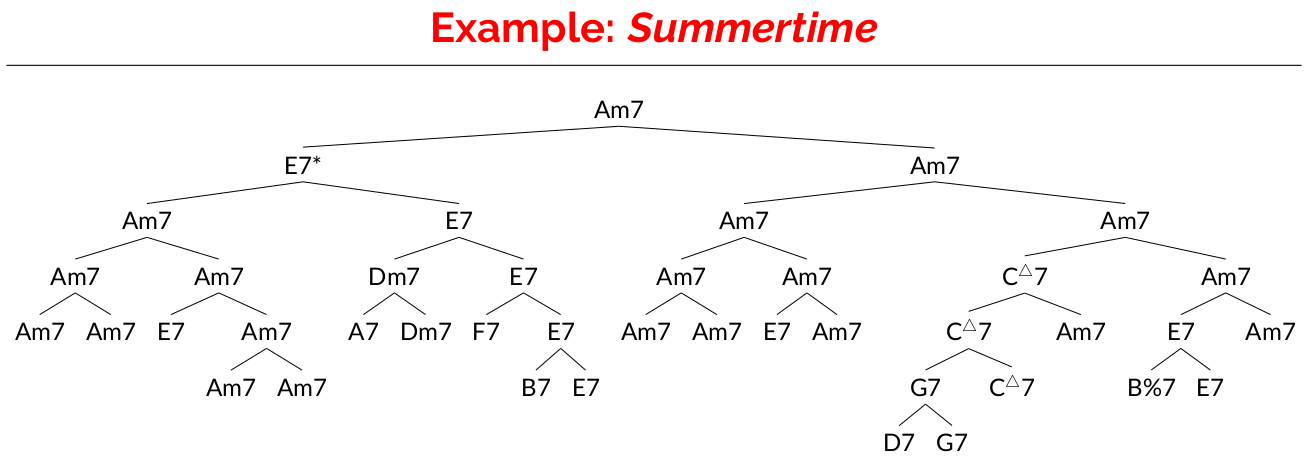
\includegraphics[height=40mm, width=120mm]{
    z_images/2_etat_de_l_art/1_summertime_tree.png}
	\caption{arbre\_jazz}
	\textit{Représentation arborescente d’une grille harmonique}
    \cite{harasimjazz}
\end{figure}
<dam>il serait mieux de citer cette figure et de la commenter un peu</dam>

\section*{Conclusion}
La plupart des travaux déjà existants sur la TAB ont été énumérés par Wu
\textit{et al.} \cite{Review_ADT} qui, pour mieux comprendre la pratique des
systèmes de TAB, se concentrent sur les méthodes basées sur la factorisation
matricielle et celles utilisant des réseaux neuronaux récurrents. La majorité
de ces recherches se concentre sur des méthodes de calcul pour la détection
d'événements sonores de batterie à partir de signaux acoustiques ou sur la
séparation entre les évènements sonores de batterie avec ceux des autres
instruments dans un orchestre ou un groupe de musique \cite{2802}, ainsi que
sur l'extraction de caractéristiques de bas niveau telles que la classe
d'instrument et le moment de l'apparition du son. Très peu d'entre eux ont
abordé la tâche de générer des partitions de batterie et, même quand le sujet
est abordé, l’output final n’est souvent qu’un fichier MIDI non-quantifié et
non une partition écrite.

%\florent{diff. pour production de partition (et 1 des obj. du stage) est...}
En conclusion, il n’existe pas de formalisation de la notation de la batterie
ni de réelle génération de partition finale, dont les enjeux principaux
seraient :
\begin{enumerate}
    \item le passage du monophonique au polyphonique, comprenant la distinction
        entre les sons simultanés et les appogiatures ou autres ornements ;
    \item les choix d’écritures spécifiques à la batterie concernant la
        séparation des voix et les continuations.
\end{enumerate}
